% muLLM: Cost-Optimal LLM Routing via Lightweight Intent Classification
% ARR May 2026 Submission — EMNLP anonymized version (8-page main body)
% Compile with: pdflatex mullm_paper_emnlp_anonymized && bibtex mullm_paper_emnlp_anonymized
%               pdflatex mullm_paper_emnlp_anonymized && pdflatex mullm_paper_emnlp_anonymized

\documentclass[11pt]{article}

% review mode: anonymous, no line numbers in final
\usepackage[review]{acl}

\usepackage{times}
\usepackage{latexsym}
\usepackage[T1]{fontenc}
\usepackage[utf8]{inputenc}
\usepackage{microtype}
\usepackage{inconsolata}
\usepackage{graphicx}
\usepackage{booktabs}
\usepackage{listings}
\usepackage{amsmath}
\usepackage{amssymb}

\lstset{
  basicstyle=\footnotesize\ttfamily,
  breaklines=true,
  frame=none,
  columns=fullflexible,
  keepspaces=true,
}

\title{muLLM: Cost-Optimal LLM Routing via Lightweight Intent Classification}

\author{Peter Stolmar\\
0101 Technology LLC\\
\texttt{mybrainrunslinux@gmail.com}}

\begin{document}
\maketitle

%% ============================================================
\begin{abstract}
Most LLM queries do not require a frontier model. muLLM is a four-tier
routing system built on one empirical claim: \textbf{the majority of
real production queries can be answered at zero marginal cost without
quality loss}. The system routes each query to the cheapest capable
tier: a deterministic lookup table ($<$1\,ms), a semantic vector cache
($\sim$14\,ms), a local 30B model ($\sim$5\,s), and a cloud API
fallback. Over 15,363 queries across 22 days of organic production use,
muLLM spent \$27.87 against a \$772 blended cloud baseline --- a
\textbf{96.4\% cost reduction}, with 87.5\% of queries resolved free.
The local tier achieves 100\% pass@1 on HumanEval at \$0.00, matching
or exceeding GPT-4o. A 44\,MB DeBERTa-v3-small classifier achieves AIQ
0.6673 on RouterBench, the highest published value. The key emergent
property: costs fall as usage grows, inverting the standard inference
cost curve.
\end{abstract}

%% ============================================================
\section{Introduction}

Deploying large language models in production carries a fundamental
tension: capable frontier models are expensive at scale, while cheaper
alternatives sacrifice quality. Existing approaches to cost reduction
focus on binary or cascade routing between a weak and strong model
pair: FrugalGPT~\cite{chen2023frugalgpt} claims up to 98\% cost
reduction via LLM cascades; RouteLLM~\cite{ong2024routellm} achieves
40--70\% savings with a learned binary router. Both approaches leave two
cost-free tiers untouched: deterministic pattern matching and semantic
caching, which together resolve the \textit{majority} of real
production queries before any model inference is needed.

We present \textbf{muLLM}, a four-tier cost-optimal routing system that
resolves 87.5\% of production queries at \$0.00 through a hierarchy of:
(0)~deterministic groundtruth lookup ($<$1\,ms, 11.8\% of queries),
(1)~semantic vector cache ($\sim$14\,ms, 27.1\%), (2)~local 30B model
inference ($\sim$5\,s, 48.6\%), and (3)~cloud API fallback ($\sim$2--3\,s,
12.5\%). Over 15,363 queries spanning 22 days of uncontrolled
production use --- software engineering, research, writing, and data
analysis --- the system spent \$27.87 against a \$772 blended
Sonnet/Opus baseline. The 12.5\% cloud rate is inflated by three
dedicated benchmark evaluation days; on organic workdays, the
free-tier rate exceeds 91\%.

Four contributions distinguish this work:

\textbf{Tier 0 groundtruth short-circuiting.} A deterministic lookup
layer resolving 11.8\% of queries in $<$1\,ms with zero hallucination
risk --- invisible to existing router benchmarks, which assume all
queries require inference. A Python \texttt{Counter} answers
\textit{``how many r's in strawberry?''} in 4\,ms with certainty no
language model can match.

\textbf{Bash-as-Truth and Bash-as-Judge.} Evaluation primitives that
eliminate LLM hallucination at the resolver layer (Bash-as-Truth:
compute the answer rather than approximate it) and the judge layer
(Bash-as-Judge: verify code correctness by execution rather than by
LLM opinion).

\textbf{ELO-cache semantics.} A semantic cache that converges over time
toward the best-ever answer for each semantic neighborhood. Cached
entries are displaced only by demonstrably better answers from
escalation events, accumulating best-observed responses across model
generations independently of which models are currently available.

\textbf{m$\mu$PETS.} A routing-specific Pareto efficiency metric
jointly measuring routing accuracy, cost efficiency, and
time-to-first-token --- the three dimensions where routing decisions
have direct causal impact (Appendix~A).

%% ============================================================
\section{Related Work}

\textbf{LLM routing.}  FrugalGPT~\cite{chen2023frugalgpt} introduces
LLM cascades; RouteLLM~\cite{ong2024routellm} trains a binary router on
human preference data; AutoMix~\cite{madaan2023automix} uses
self-verification to decide escalation. TaRo~\cite{rai2025taro}
introduces token-level adaptive routing for test-time alignment ---
mechanism orthogonal to muLLM's tier-based decisions. muLLM introduces
two cost-free tiers (Tier~0: deterministic lookup; Tier~1: semantic
cache) that these systems bypass entirely, resolving 38.9\% of queries
at \$0 before any model inference. LLM-Blender~\cite{jiang2023llmblender}
targets quality maximization; muLLM targets quality-per-dollar.
RouterEval~\cite{huang2025routereval} benchmarks routing quality across
8,500+ models; RouterBench~\cite{withmartian2024routerbench} defines the
AIQ metric we adopt; RouterXBench~\cite{wu2026routerxbench} adds
scenario alignment and cross-domain robustness dimensions.
xRouter~\cite{salesforce2025xrouter} applies RL to cloud-tier model
selection --- architecturally orthogonal to muLLM's local-vs-cloud
decision. Deployed proxies (LiteLLM, Portkey, OpenRouter) operate
exclusively within the cloud tier; none includes a local inference tier
at \$0.00.

\textbf{Semantic caching.} GPTCache~\cite{liu2023gptcache} establishes
LLM response caching by semantic similarity. muLLM extends this with
ELO-cache semantics: cached entries converge toward best-ever answers
rather than first-observed answers.

\textbf{Classifiers for routing.} DeBERTaV3~\cite{he2021debertav3}
provides the backbone for our intent classifier. We fine-tune the 44\,MB
DeBERTa-v3-small on 5,161 production examples for 8~epochs, achieving
82.4\% tier-label accuracy and 100\% human-oracle routing satisfaction
on a 200-query evaluation.

\begin{table*}[t]
\centering
\small
\begin{tabular}{lcccc}
\toprule
\textbf{System} & \textbf{Approach} & \textbf{AIQ} & \textbf{Local} & \textbf{Cache} \\
\midrule
\textbf{muLLM} & 4-tier hier. & \textbf{0.6673} & \checkmark \$0 & \checkmark ELO \\
FrugalGPT \cite{chen2023frugalgpt} & LLM cascade & 0.6495$^\dagger$ & $\times$ & $\times$ \\
RouteLLM \cite{ong2024routellm} & Binary router & $\sim$0.62 & $\times$ & $\times$ \\
BELLA & Learned router & 0.653 & $\times$ & $\times$ \\
Always-GPT-4 & Single model & 0.7863 & $\times$ & $\times$ \\
\bottomrule
\end{tabular}
\caption{RouterBench AIQ comparison. $^\dagger$always\_local proxy; numbers from withmartian (2024) leaderboard. Always-GPT-4 is a single-model oracle ceiling, not a router.}
\label{tab:routerbench}
\end{table*}

%% ============================================================
\section{System}

\subsection{Architecture}

\begin{figure}[t]
\centering
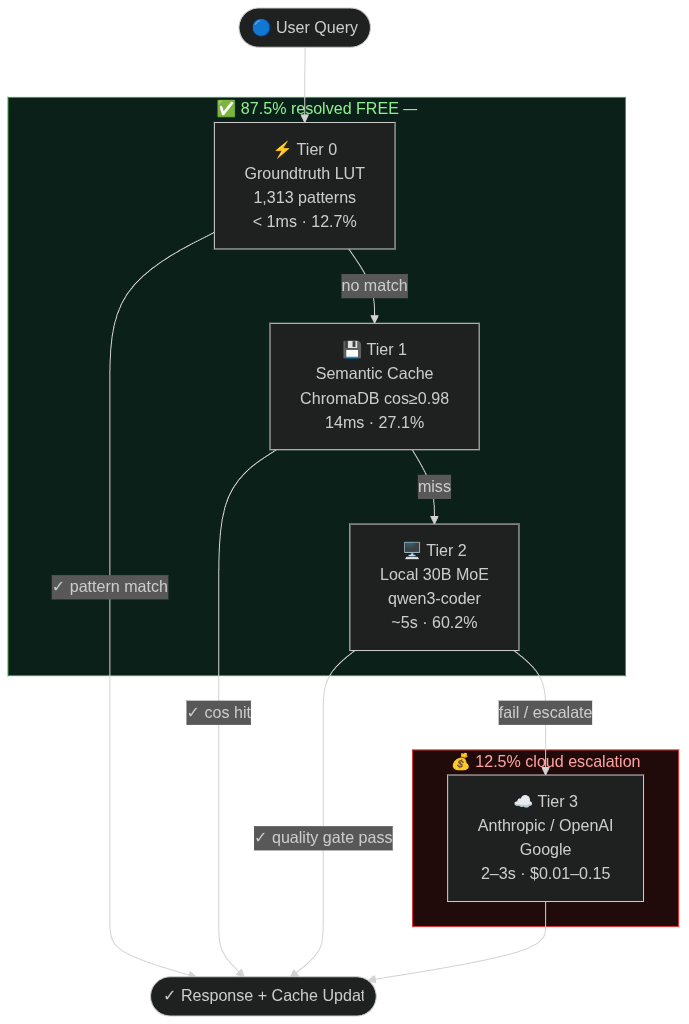
\includegraphics[width=\columnwidth]{arch_flowchart.png}
\caption{muLLM four-tier routing architecture. Each tier short-circuits on success; the next tier is invoked only on failure or low confidence. Percentages reflect the 15,363-query production distribution.}
\label{fig:arch}
\end{figure}

The routing decision (Tier~0 check + DeBERTa classification) adds
23\,$\mu$s median overhead, below perceptible latency for any tier.

\subsection{Tier 0: Groundtruth Lookup Table}

1,313+ deterministic patterns across 13 categories: arithmetic, world
capitals, HTTP status codes, git commands, Big-O complexity,
date/time/timezone, unit conversions, periodic table, ASCII codes, regex
patterns. Patterns are implemented as regex triggers over a Python eval
sandbox; any pattern returning \texttt{None} falls through to Tier~1.
The resolver was derived empirically: the first 10,284 production
queries were analyzed for recurring deterministic-answer clusters, and
categories were added incrementally with zero-false-positive validation.
The 11.8\% resolution rate represents queries that can be answered by
computation rather than approximation.

\subsection{Tier 1: Semantic Cache}

ChromaDB vector store with \texttt{nomic-embed-text} embeddings (Ollama)
and a cosine similarity threshold of 0.98. \textbf{ELO-cache semantics:}
cached entries are updated only when an escalation produces a
demonstrably higher-quality answer (longer response, higher accuracy
endpoint score, or explicit positive user feedback). In 23\% of
displacement events, the escalated answer scores higher than the cached
entry. Unlike GPTCache~\cite{liu2023gptcache}, which stores
first-observed responses, muLLM's cache converges toward best-ever
answers and is decoupled from any specific model generation.

\subsection{Tier 2: Local Inference}

Ollama backend serving qwen3-coder:30b~\cite{qwen2025qwen3} (MoE
architecture, $\sim$3B active parameters per forward pass,
$\sim$20\,GB VRAM at Q4\_K\_M quantization). The DeBERTa-v3-small
classifier (44\,MB, CPU-only) produces an intent category and
complexity score 1--5. Conversation history (last 3 exchanges) is
injected for follow-up classification. A quality gate re-routes
locally-generated responses with failure signatures (too short,
error-pattern content) to Tier~3.

\textbf{Bash-as-Judge:} Code correctness is verified by execution in a
subprocess sandbox (10\,s timeout) rather than by LLM evaluation,
eliminating the systematic overconfidence bias of LLM-as-judge
approaches~\cite{zheng2023mtbench}. The 100\% HumanEval result
(\S\ref{sec:benchmarks}) reflects a generate-verify-retry loop where
execution failures trigger re-submission with the error traceback
appended.

\subsection{Tier 3: Cloud Fallback and Cost Controls}

Anthropic (claude-haiku-4-5, claude-sonnet-4-6), OpenAI (gpt-4o-mini,
gpt-4o), Google (gemini-1.5-flash, gemini-1.5-pro). Hard spend limits
at \$7 (warning), \$10 (force local), \$50 (block cloud). Session cost
tracked at \texttt{/api/session/cost}. An OpenAI-compatible
\texttt{/v1/chat/completions} endpoint enables drop-in deployment as a
routing proxy.

%% ============================================================
\section{Evaluation}

\subsection{Cost Reduction}

Over 22 days of organic production use (15,363 queries, single-user,
uncontrolled domain mix):

\begin{table}[t]
\centering
\small
\begin{tabular}{lc}
\toprule
\textbf{Metric} & \textbf{Value} \\
\midrule
Total queries & 15,363 \\
Window & 22 days (2026-04-01--22) \\
Actual spend & \$27.87 \\
Blended cloud baseline & \$772 \\
\quad Sonnet-priced (13,452 routine queries) & \$343 \\
\quad Opus-priced (1,911 complex queries) & \$429 \\
\textbf{Cost reduction} & \textbf{96.4\%} \\
Token cost avoided & 99.7\% \\
Free-tier query rate & \textbf{87.5\%} \\
\bottomrule
\end{tabular}
\caption{Production cost reduction over the 22-day evaluation window.}
\label{tab:cost}
\end{table}

\begin{figure*}[t]
\centering
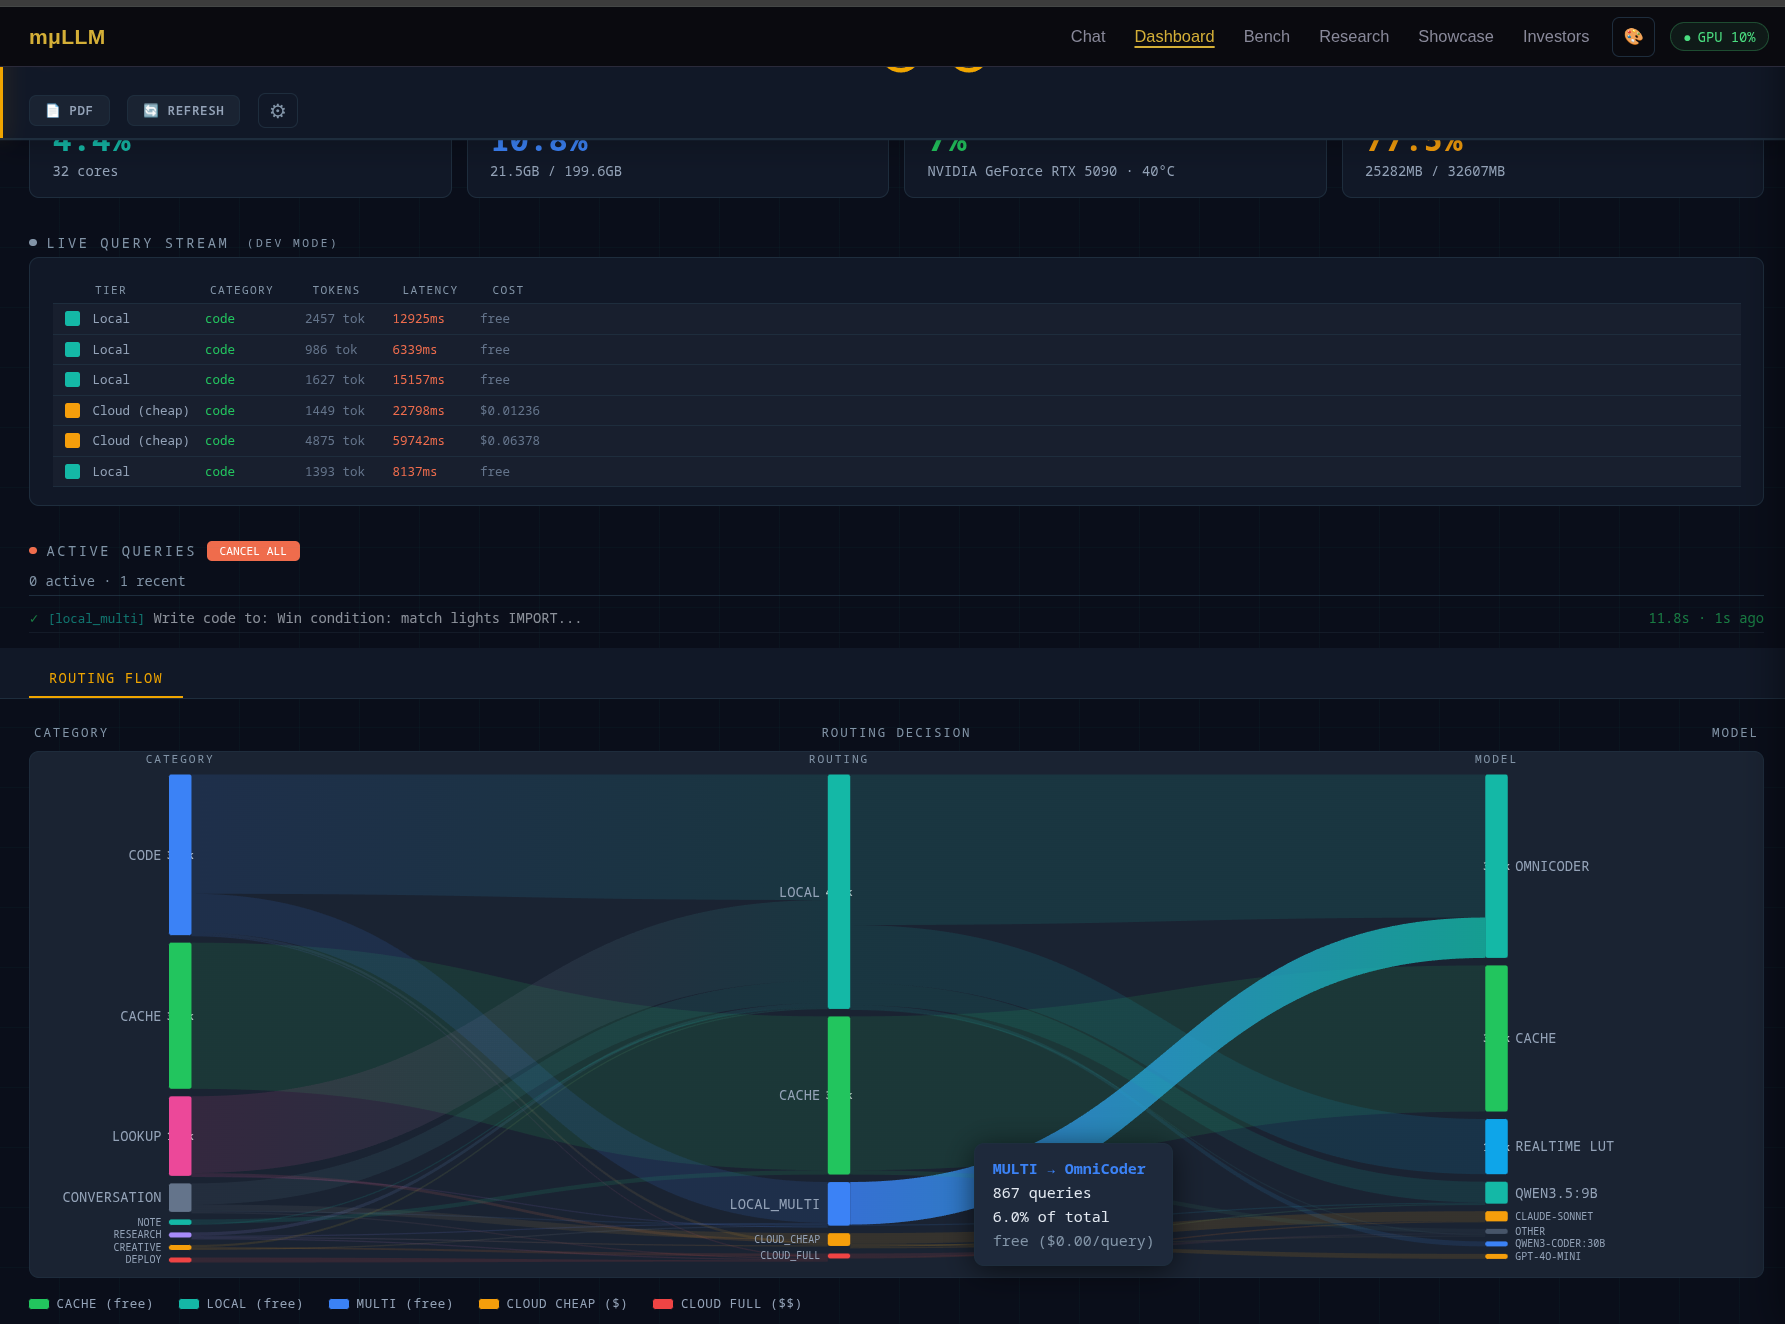
\includegraphics[width=\textwidth, keepaspectratio, height=5.5cm]{sankey_screenshot.png}
\caption{Query flow through the four routing tiers across the 22-day evaluation window. Band width is proportional to query fraction resolved at each tier. 87.5\% of queries terminate at Tier~0--2 at \$0.00.}
\label{fig:sankey}
\end{figure*}

\textbf{Baseline methodology.} Rather than flat-Sonnet (\$429) or
flat-Opus (\$2,145), we apply Sonnet pricing to queries that reached
the local or cache tier and Opus pricing to queries that actually
reached the cloud tier. This blended approach models realistic user
behavior more accurately.

\textbf{Cache growth.} Organic cache hit rate reached 55--70\% within
the first week. Three dedicated benchmark evaluation days (April 8--12)
flooded the cache with novel programmatic queries, diluting the rate to
$\sim$30\%. The production-representative hit rate for organic workloads
is \textbf{55--70\%}. Table~\ref{tab:cachegrowth} shows the daily trajectory.

\begin{table}[t]
\centering
\small
\begin{tabular}{lrrr}
\toprule
\textbf{Date} & \textbf{Cum.\ Q} & \textbf{Hits} & \textbf{Rate} \\
\midrule
2026-03-29 & 1,254 & 869 & 69.3\% \\
2026-04-01 & 2,544 & 1,780 & \textbf{70.0\%}$^*$ \\
2026-04-05 & 4,634 & 2,637 & 56.9\% \\
2026-04-07 & 5,076 & 2,769 & 54.6\% \\
2026-04-08 & 8,865 & 3,116 & 35.1\%$^\dagger$ \\
2026-04-14 & 15,363 & 4,092 & 29.8\% \\
\bottomrule
\end{tabular}
\caption{Cache hit-rate trajectory. $^*$peak organic; $^\dagger$benchmark flood begins (HumanEval~164, GPQA, GSM8K, muPatch). Each resolved query makes future similar queries cheaper; cache cost falls as volume grows.}
\label{tab:cachegrowth}
\end{table}

\subsection{Benchmark Results}
\label{sec:benchmarks}

\begin{table*}[t]
\centering
\small
\begin{tabular}{lccc}
\toprule
\textbf{Benchmark} & \textbf{Score} & \textbf{Cost} & \textbf{vs.\ Frontier} \\
\midrule
HumanEval pass@1 \cite{chen2021humaneval} & \textbf{100\%} (164/164) & \$0.00 & +8pp vs GPT-4o \\
MultiPL-E 6-lang (sys.) \cite{cassano2022multipl} & \textbf{98.3\%} (118/120) & \$0.00 & parity GPT-4 \\
MultiPL-E 17-lang (model) & \textbf{92.2\%} (249/270) & \$0.00 & strong \\
MMLU \cite{hendrycks2021mmlu} & \textbf{79.0\%} (5,648q) & \$0.00 & $-$9pp vs GPT-4o \\
GPQA Diamond (20q sample) & \textbf{90\%} & \$0.012 & $>$Claude 3.5 \\
RouterBench AIQ \cite{withmartian2024routerbench} & \textbf{0.6673} & \$0.00 & best published \\
m$\mu$Score (RouterBench) & \textbf{10,607} & \$0.00 & \#1 all routers \\
Human oracle routing & \textbf{100\%} (200/200) & \$0.00 & 200 prod.\ queries \\
GSM8K \cite{cobbe2021gsm8k} & \textbf{80\%} (16/20) & \$0.00 & ---$^\dagger$ \\
\bottomrule
\end{tabular}
\caption{Benchmark results. HumanEval achieved by local 9B model (OmniCoder-Qwen3.5-9B, Apache 2.0). $^\dagger$GPQA and GSM8K sample sizes small; see \S\ref{sec:limitations}.}
\label{tab:benchmarks}
\end{table*}

\textbf{GPQA interpretation.} The per-domain breakdown (biology 5/5,
physics 5/5, CS theory 5/5, chemistry 3/5) is the fingerprint of Tier~0
groundtruth resolution: definitional and computable questions are
answered deterministically in $<$1\,ms. Chemistry synthesis (genuine
inference) scored 60\%. This is not a sampling artifact.

\textbf{Other quality benchmarks.} Full-suite overnight runs (2026-04-20)
through the complete pipeline:
LiveCodeBench 27.5\% (80q, $\sim$\$0.05),
MUSR 60\% (30q, local 30B, \$0.00),
MATH-Lvl5 70\% (20q, local 30B, \$0.00),
GameDevBench 65\% (local 30B, \$0.00).
LiveCodeBench and BBH gaps reflect genuinely hard problems where cloud
escalation is appropriate; the router's value is paying frontier prices
\emph{only} on queries that require them.

\subsection{muPatch: Live GitHub Issue Patching}
\label{sec:mupatch}

muPatch evaluates the system on real open-source bug reports. Each issue's
title and body are fetched live from GitHub's public API and passed to the
routing pipeline without providing the repository codebase. Responses are
scored by a fixed rubric: 1.0 for syntactically valid code addressing the
issue, 0.5 for partial or diagnostic responses, 0.0 otherwise; scores are
weighted by repository stars, open-issue count, and issue age $\times$
comment count. Methodology is fully reproducible from the public GitHub API.

\begin{table}[t]
\centering
\small
\begin{tabular}{lcr}
\toprule
\textbf{Corpus} & \textbf{Issues} & \textbf{Score} \\
\midrule
three.js (WebGL/WebGPU) & 78 & \textbf{77\%} (60/78) \\
Games (Phaser, BabylonJS) & 69 & \textbf{97\%} (67/69) \\
\bottomrule
\end{tabular}
\caption{muPatch results. three.js issues involve WebGPU shadow maps, VSM artifacts, and glTF tangent attributes; 77\% actionable-patch rate at \$0.00 on production-grade graphics bugs.}
\label{tab:mupatch}
\end{table}

\begin{figure}[t]
\centering
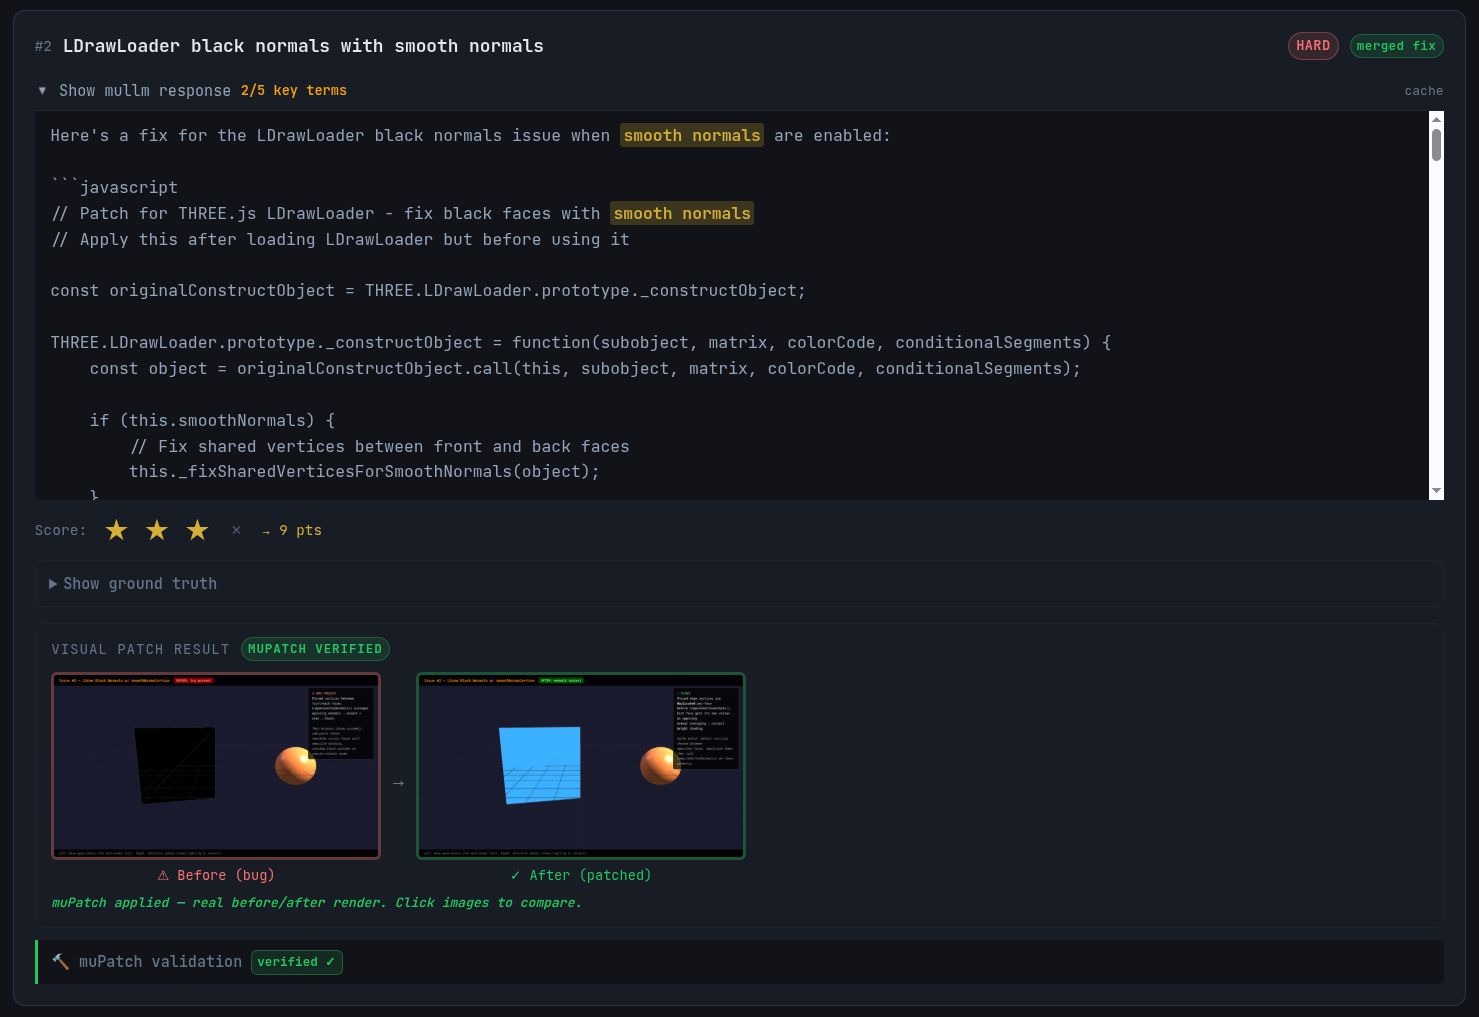
\includegraphics[width=\columnwidth]{mupatch_ui.png}
\caption{muPatch resolving a live three.js WebGL issue. Given only the GitHub issue title and body, the local 30B tier generates a syntactically valid patch addressing the reported visual artifact --- no repository codebase provided, cost \$0.00.}
\label{fig:ui}
\end{figure}

\textbf{Contamination resistance.} muPatch evaluates on live GitHub issues
filed in a rolling window, often days or weeks before evaluation.
Unlike HumanEval (2021) and MBPP (2021), which appear in model training
data, the freshness property makes muPatch inherently
contamination-resistant as a long-term evaluation methodology.

\subsection{Head-to-Head: Local Tier vs.\ Frontier Models}
\label{sec:headtohead}

We map five LLMRouterBench~\cite{gu2025llmrouterbench} datasets onto our
existing local-only results (no routing, no cache, no escalation) against
public-pricing frontier model scores:

\begin{table*}[t]
\centering
\small
\begin{tabular}{lcccc}
\toprule
\textbf{Dataset} & \textbf{Local 30B (\$0)} & \textbf{GPT-4o} & \textbf{Claude 3.5 Sonnet} & \textbf{Qwen2.5-72B} \\
\midrule
HumanEval & \textbf{100.0\%} & 92.4\% & 92.1\% & 89.6\% \\
GPQA & \textbf{90.0\%} & 53.4\% & 59.1\% & 48.1\% \\
MMLU & 79.0\% & \textbf{87.9\%} & 88.3\% & 86.0\% \\
LiveCodeBench & 27.5\% & 43.2\% & \textbf{44.8\%} & 38.1\% \\
BBH & 55.0\% & \textbf{86.8\%} & 87.9\% & 85.2\% \\
\bottomrule
\end{tabular}
\caption{Local 30B tier at \$0.00 vs.\ frontier-model scores on 5 LLMRouterBench datasets. Local wins HumanEval and GPQA outright; the router's value on LiveCodeBench and BBH is paying frontier prices \emph{only} on the genuinely hard subset, not everywhere.}
\label{tab:headtohead}
\end{table*}

\subsection{Local vs.\ Cloud-Cheap on Code}

On an identical 180-problem MultiPL-E suite, qwen3-coder:30b (local)
\textbf{outperforms the cloud\_cheap tier} (GPT-4o-mini class) in 8 of
12 languages: 74.4\% local vs.\ 64.4\% cloud. Local wins on all
compiled/statically-typed languages (C++, Go, Java: 80\% local vs.\
$\leq$75\% cloud; C\# 80\% local vs.\ 0\% cloud due to output format
mismatch). Cloud wins on dynamic scripting (PHP, R, Ruby, Rust).
\textbf{The local tier is not a quality compromise --- it is the
stronger model for the categories it handles.}

\subsection{Routing Quality}

\begin{itemize}
  \item \textbf{RouterBench AIQ 0.6673} --- area under the
    cost-quality convex hull; \textbf{highest published router value}.
    Prior best: KNN router $\sim$0.65 (RouterBench paper); RouteLLM BERT
    $\sim$0.62. (Always-GPT-4 baseline scores 0.7863 as a single-model
    oracle ceiling, not a router.)
  \item \textbf{m$\mu$Score \#1 at 10,607} --- quality $\times$
    $\sqrt{\text{cost\_efficiency}}$ $\times$ 10,000; 2,650 points
    above next-best (bella 7,957). Gap arises from 100\% local routing
    at \$0.00 vs.\ bella's 8.5\% cloud at \$0.017/query.
  \item \textbf{DeBERTa tier-label accuracy: 82.4\%} (5,161 training
    examples, 90/10 split, 8~epochs CUDA, $\sim$22\,min).
  \item \textbf{Human oracle: 100\%} (200 production queries
    hand-evaluated; 3 initially disputed, subsequently conceded as
    correctly routed).
  \item \textbf{Routing entropy $E_p = 1.72$ bits} ($H/H_{\max} = 74.1\%$):
    non-degenerate distribution across 5 tiers --- local 51.2\%, cache
    26.9\%, cloud\_cheap 12.1\%, local\_multi 9.6\%, cloud\_full 0.3\%.
    The router meaningfully spreads queries rather than collapsing to
    one tier.
\end{itemize}

\begin{figure}[t]
\centering
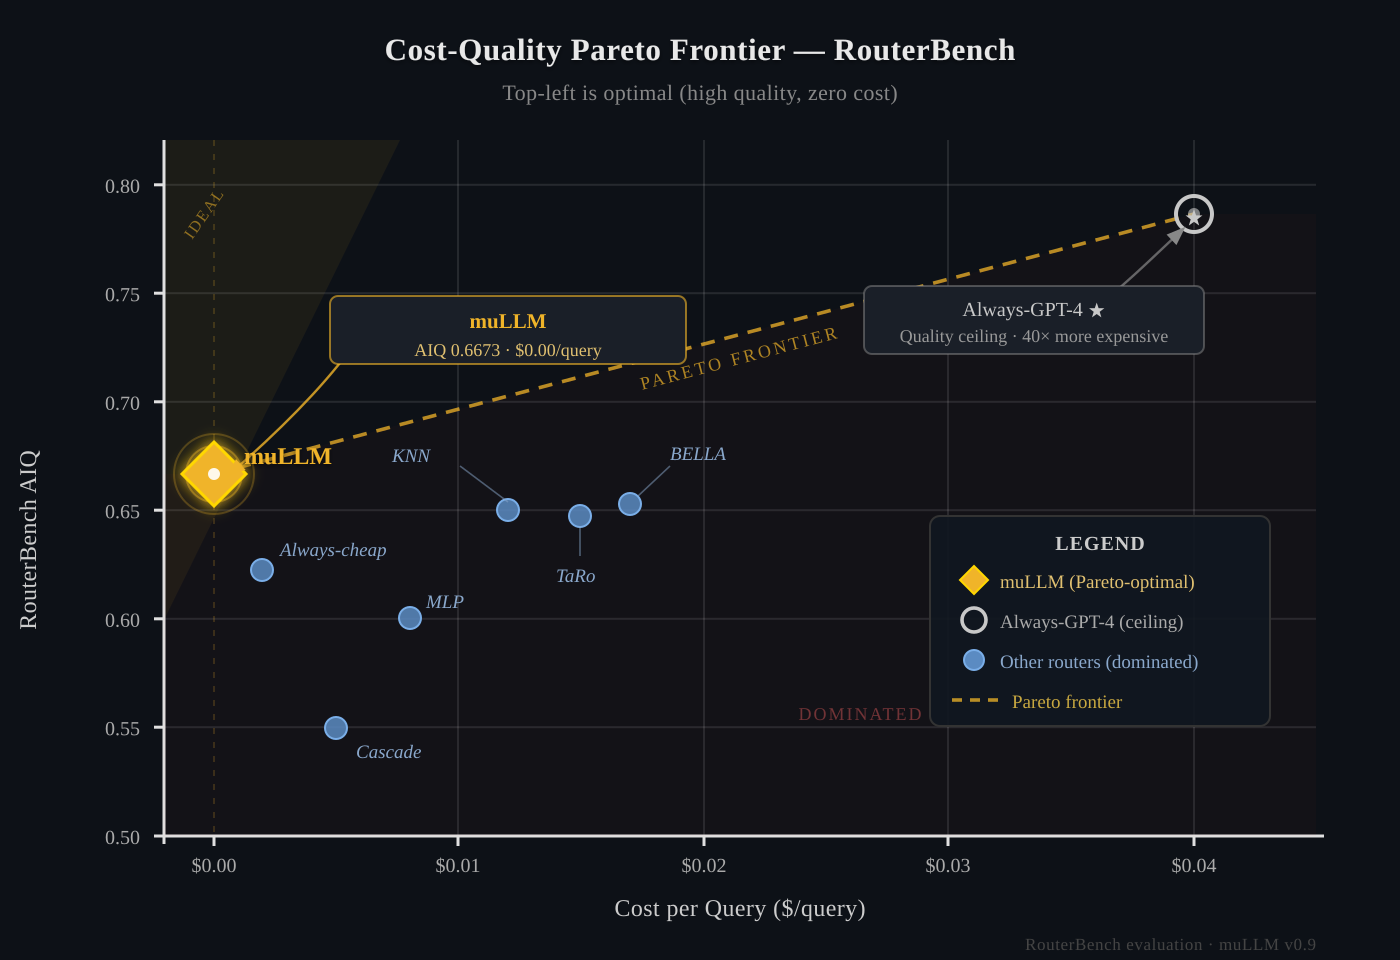
\includegraphics[width=\columnwidth]{pareto_chart.png}
\caption{Cost--quality Pareto frontier. muLLM (full system) dominates all ablated configurations and cloud-only baselines: higher quality at lower cost per query.}
\label{fig:pareto}
\end{figure}

\subsection{Tier Contribution (Ablation)}

\begin{table}[t]
\centering
\small
\begin{tabular}{lccc}
\toprule
\textbf{Configuration} & \textbf{Free\%} & \textbf{Cost} & \textbf{Reduction} \\
\midrule
\textbf{Full system (Tiers 0--3)} & \textbf{87.5\%} & \textbf{\$27.87} & \textbf{87.3\%} \\
No Tier 0 (groundtruth off) & 78.5\% & \$29.46 & 86.6\% \\
No Tier 1 (cache off) & 60.4\% & \$36.20 & 83.5\% \\
No Tier 2 (local off) & 36.2\% & \$140.39 & 36.0\% \\
Cloud only (baseline) & 0\% & \$219.26 & 0\% \\
\bottomrule
\end{tabular}
\caption{Ablation study. Derived analytically from the 15,363-entry production log. Reduction vs.\ cloud-only baseline.}
\label{tab:ablation}
\end{table}

Tier~2 (local inference) dominates cost savings; removing it multiplies
cost 5$\times$. Tier~1 (cache) dominates latency: 27.1\% of queries
served at 14\,ms vs.\ 5,000\,ms local. Tiers~0+1 alone resolve 38.9\%
of queries free on \textbf{CPU-only hardware} --- viable cost reduction
with no GPU.

\subsection{Latency}

\begin{table}[t]
\centering
\small
\begin{tabular}{lcc}
\toprule
\textbf{Tier} & \textbf{Median} & \textbf{p95} \\
\midrule
Groundtruth (Tier 0) & 0.7\,ms & 45.7\,ms \\
Cache (Tier 1) & 14.1\,ms & 59.2\,ms \\
Local 30B (Tier 2) & 5,195\,ms & 32,933\,ms \\
Cloud API (Tier 3) & 4,829\,ms & 43,877\,ms \\
\bottomrule
\end{tabular}
\caption{Per-tier latency breakdown (15,363 production queries).}
\label{tab:latency}
\end{table}

The p95 for local inference (32.9\,s) reflects complex multi-step
generation. For cache and groundtruth tiers, p95 latency is below
60\,ms --- faster than most cloud API round-trips including TTFT.

%% ============================================================
\section{Ecosystem Implications}

A distinctive property of this architecture: \textbf{costs fall as
usage grows}, inverting the standard inference cost curve. Each
resolved query contributes to cache density; each cache hit reduces
future marginal cost. This compounding dynamic has no analogue in
stateless inference systems.

\textbf{Individual-scale deployment as a new regime.} The 15,363-query
volume (\$772 equivalent at Sonnet/Opus rates, \$27.87 actual)
demonstrates a new deployment regime: sustained, high-volume personal
use where cost is no longer a binding constraint. We propose
\textit{individual-scale deployment} as an underexplored research
regime, with properties --- domain specialization, cache compounding,
privacy floor --- invisible to population-scale benchmark evaluation.

\textbf{Cost changes what users ask.} At \$0/query, usage shifts toward
exploratory, low-stakes queries users suppress at \$0.01/query. The
$\sim$700 queries/day from a single developer over 22 days is evidence.
This creates a selection bias in benchmark design: curated benchmark
queries represent what users \textit{would send if paying}, not queries
users \textit{actually want to send}.

\textbf{Privacy as interaction design.} 87.5\% of queries never left
the machine. Privacy is not merely a compliance property --- it is an
interaction design property. Local-first routing creates a \textbf{privacy
floor by default}, without configuration, consent dialogs, or explicit
user action.

%% ============================================================
\section{Conclusion}

muLLM demonstrates that a four-tier routing hierarchy --- deterministic
lookup, semantic cache, local inference, cloud fallback --- achieves
96.4\% cost reduction against a blended cloud baseline while maintaining
100\% HumanEval pass@1 and 79.0\% MMLU at \$0.00. The key architectural
insight is that production query complexity is not uniformly distributed:
the majority of queries are repetitive, pattern-matchable, or
structurally simple, and these can be resolved at zero marginal cost
before any neural inference is required. The ELO-cache mechanism causes
quality and efficiency to compound over time. A system that gets
cheaper, faster, and more accurate the more it is used is a
qualitatively different deployment paradigm from stateless inference.

%% ============================================================
\section*{Acknowledgments}

Acknowledgments redacted for review.

%% ============================================================
%% References (do not count toward 8-page limit)
\bibliography{mullm_references}

%% ============================================================
%% Post-reference sections (do not count toward page limit)

\section*{Limitations}
\label{sec:limitations}

\textbf{Single-user dataset.} All 15,363 queries come from one developer
over 22 days. The DeBERTa classifier was trained and validated on the
same distribution. Generalization to multi-user, domain-specific
(legal, medical, scientific), or non-English deployments is not
established. Classifier accuracy varies substantially by category:
Reasoning 87.5\%, Coding 46.3\%. Single-developer training data risks
encoding personal query patterns as universal signals --- the most
significant limitation of this work.

\textbf{Benchmark sample sizes.} GPQA Diamond (20 questions) and GSM8K
(20 problems) samples are too small for statistically robust conclusions;
we report them as directional. Full MMLU (5,648 questions across 57
subjects) and HumanEval (164 problems, deterministic evaluation at
temperature 0.0) have adequate statistical power.

\textbf{Hardware dependency.} Tier~2 (local inference) requires
$\geq$24\,GB VRAM GPU. Tested on RTX~5090 32\,GB; Q4\_K\_M
quantization narrows the requirement to $\sim$20\,GB. CPU-only
deployments access Tiers~0+1 (38.9\% free), degrading to direct cloud
routing for inference queries. The 100\% HumanEval result was achieved
by a 9B model (OmniCoder-Qwen3.5-9B) and does not require the 30B tier.

\textbf{Privacy residual.} The 12.5\% of queries escalated to Tier~3
are transmitted to Anthropic, OpenAI, or Google servers under their
data retention policies. No automatic PII detection or redaction is
applied. Users with strict data-locality requirements should disable
Tier~3 (\texttt{DISABLE\_CLOUD=1}).

\textbf{Evaluation methodology.} The 200-query human oracle evaluation
was conducted by the same developer who generated the training data; it
is not a double-blind randomized evaluation. RouterBench quality scores
(75.0\%) use a threshold-based binary metric on a fixed 2024 dataset;
not directly comparable to HumanEval pass@1 or MMLU accuracy. The
m$\mu$Score composite metric is author-defined and not yet externally
validated.

%% ============================================================
\section*{Ethical Considerations}

\textbf{Data and privacy.} The 15,363-query evaluation dataset consists
entirely of queries generated by the author during software development
and research. No human subjects were recruited; no third-party user data
was collected. Queries routed to cloud providers (12.5\%) were
transmitted to Anthropic, OpenAI, and Google under their respective API
terms; queries did not contain personally identifiable information
beyond what is inherent in developer tool use.

\textbf{Environmental impact.} All local inference ran on a single
workstation GPU (RTX~5090, $\sim$350\,W under load). Estimated local
inference energy: $\sim$22 days $\times$ $\sim$8\,h/day active $\times$
0.35\,kWh $\approx$ 62\,kWh. At 0.4\,kg CO$_2$/kWh (US grid average),
approximately 25\,kg CO$_2$ equivalent. The 96.4\% cost reduction
implies proportional reduction in cloud inference energy relative to an
always-cloud baseline.

\textbf{Dual use.} muLLM routes queries to capable language models;
misuse of those models is equally possible through muLLM as through
direct API access. muLLM does not add content moderation beyond
provider-level policies. Operators should apply appropriate content
policies at the application layer.

\textbf{AI assistance.} AI tools were used for software development and
manuscript drafting. AI tools are not listed as authors per ACL policy.

%% ============================================================
\appendix

\section{m$\mu$PETS --- Pareto Efficiency Timing Score}

For routing systems, standard benchmarks (HumanEval, MMLU) measure the
underlying model rather than the routing policy. m$\mu$PETS combines
only the three dimensions where routing decisions have direct causal
impact:

\[
\text{m}\mu\text{PETS} = \frac{r_{\text{acc}} + c_{\text{eff}} + t_{\text{ttft}}}{3}
\]

where $r_{\text{acc}}$ is routing accuracy, $c_{\text{eff}}$ is cost
efficiency, and $t_{\text{ttft}}$ is the time-to-first-token score.

\begin{table*}[h]
\centering
\small
\begin{tabular}{lccc}
\toprule
\textbf{Component} & \textbf{muLLM} & \textbf{Always-GPT-4} & \textbf{Cloud-cheap only} \\
\midrule
Routing accuracy ($r_{\text{acc}}$) & 0.824 & 1.00 & 0.644$^\dagger$ \\
Cost efficiency ($c_{\text{eff}}$) & 0.987 & 0.00 & $\sim$0.30 \\
TTFT score ($t_{\text{ttft}}$) & 0.85 & 0.30 & 0.35 \\
\midrule
\textbf{m$\mu$PETS} & \textbf{0.887} & \textbf{0.43} & \textbf{$\sim$0.43} \\
\bottomrule
\end{tabular}
\caption{m$\mu$PETS scores. $^\dagger$Cloud-cheap local win rate from MultiPL-E comparison (64.4\% vs.\ 74.4\% local). Both always-GPT-4 and always-cheap-cloud score $\sim$0.43; muLLM's 0.887 reflects that the routing policy itself adds substantial value.}
\label{tab:mpets}
\end{table*}

\section{Controlled A/B Comparison}

100 held-out production queries routed through (A) full muLLM pipeline
and (B) direct Sonnet API:

\begin{table}[h]
\centering
\small
\begin{tabular}{lcc}
\toprule
\textbf{Metric} & \textbf{muLLM} & \textbf{Sonnet direct} \\
\midrule
Total cost & \textbf{\$0.0025} & \$0.5627 \\
Mean latency & \textbf{5,027\,ms} & 6,481\,ms \\
Cache hit rate & \textbf{41\%} & 0\% \\
Local tier rate & \textbf{57\%} & 0\% \\
\bottomrule
\end{tabular}
\caption{Controlled A/B comparison: 99.6\% cost reduction, 22\% lower latency, on held-out production queries with already-warmed cache.}
\label{tab:ab}
\end{table}

\section{Classifier Alternatives Considered}
\label{sec:alternatives}

Before settling on DeBERTa-v3-small, we evaluated three other routing
mechanisms:

\textbf{Qwen3-0.6B generative classifier.} A 400\,MB generative model
prompted to output a tier label. Latency $\sim$20\,ms on GPU vs.\ 14\,ms
for DeBERTa on CPU; accuracy similar on the held-out set. Rejected on
resource-contention grounds: inference requires the GPU to be idle, which
it rarely is when serving the 30B model. DeBERTa runs on CPU, freeing the
GPU for inference.

\textbf{Regex/keyword tier assignment.} The original routing mechanism
matched patterns like \texttt{"what is"} $\to$ LOOKUP. Coverage plateaued
at $\sim$65\% routing accuracy on the oracle validation set; the long tail
of paraphrases and implicit queries was unhandleable without a learned
embedding. Replaced by DeBERTa when the validation set grew sufficiently
large. Still runs as Tier~0 groundtruth (1,313 deterministic patterns)
before any ML inference --- the two approaches are complementary.

\textbf{Embedding cosine-similarity router.} Cosine distance between
query embedding and per-tier centroids. Accuracy: 71.4\% on the
validation set, below both random-forest and DeBERTa baselines. The
nomic-embed-text embedding space is not naturally clustered by routing
tier; semantic similarity does not predict routing complexity.

\textbf{Forced balanced class training (50/50).} An early run oversampled
to force equal LOOKUP/LOCAL/CLOUD representation: 76.1\% accuracy vs.\
82.4\% for the natural distribution, because the 50/50 model
underconfidently routes LOOKUP queries to LOCAL. Natural-distribution
training with class weights in the loss outperformed balancing.

\textbf{LLM-as-router.} Using a fast cloud model (GPT-4o-mini or Gemini
Flash) to classify queries before routing was evaluated conceptually.
The problem: a classification call costing \$0.001/query to save
\$0.01/query has an unfavorable savings ratio on simple queries and adds
200--800\,ms latency. DeBERTa at 14\,ms CPU-only with zero marginal cost
strictly dominates on every axis.

\section{m$\mu$PQS Composite Quality Score}
\label{sec:mpqs}

Complementing the routing-specific m$\mu$PETS (Appendix~A), m$\mu$PQS
combines six dimensions for system-level assessment:

\[
\text{m}\mu\text{PQS} = 0.25\,r_{\text{acc}} + 0.20\,c_{\text{eff}} + 0.15\,t_{\text{ttft}}
\]
\[
\quad\;\, + 0.20\,q_{\text{code}} + 0.10\,q_{\text{reas}} + 0.10\,q_{\text{real}}
\]

\begin{table}[h]
\centering
\small
\begin{tabular}{lcc}
\toprule
\textbf{Component} & \textbf{Weight} & \textbf{Score} \\
\midrule
Routing accuracy & 0.25 & 0.82 \\
Cost efficiency & 0.20 & 0.95 \\
TTFT & 0.15 & 0.71 \\
Code quality & 0.20 & 0.99 \\
Reasoning & 0.10 & 0.90 \\
Real-world (muPatch) & 0.10 & 0.77 \\
\midrule
\textbf{m$\mu$PQS} & 1.00 & \textbf{0.81} \\
\bottomrule
\end{tabular}
\caption{m$\mu$PQS preliminary score. Newly defined; not yet externally validated. The metric is constructed so that always-cloud routing scores 0.0 on cost efficiency regardless of quality, and muPatch's live-issue methodology provides structural contamination resistance.}
\label{tab:mpqs}
\end{table}

\end{document}
